\documentclass{standalone}

\usepackage{pgfplots}
\pgfplotsset{compat=newest}

\begin{document}
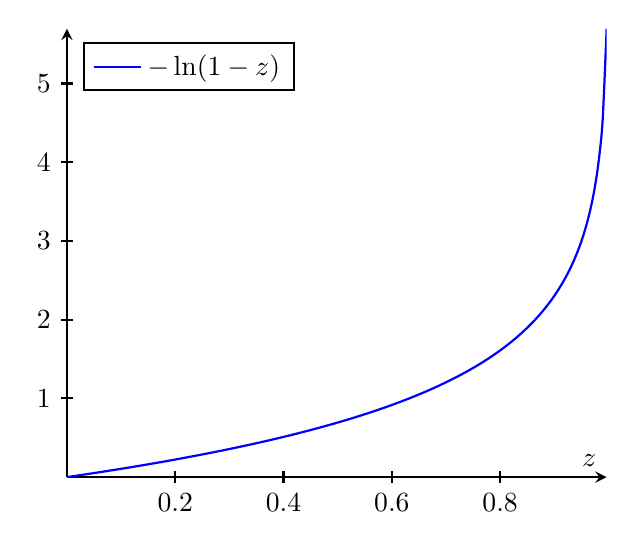
\begin{tikzpicture}
  \begin{axis}[
      xlabel = $z$,
      smooth,thick,
      axis lines = center,
      every tick/.style = {thick},
      legend pos=north west]

    \addplot[color=blue,domain=0:1.1,samples=150]{-ln(1-x)};
    \legend{$-\ln(1 - z)$}

  \end{axis}
\end{tikzpicture}
\end{document}
